\documentclass[titlepage,a4paper]{article}

\usepackage{a4wide}
\usepackage[colorlinks=true,linkcolor=black,urlcolor=blue,bookmarksopen=true]{hyperref}
\usepackage{bookmark}
\usepackage{fancyhdr}
\usepackage[spanish]{babel}
\usepackage[utf8]{inputenc}
\usepackage[T1]{fontenc}
\usepackage{graphicx}
\usepackage{float}
\usepackage{fancyvrb}

\pagestyle{fancy} % Encabezado y pie de página
\fancyhf{}
\fancyhead[L]{TP1 Java - Federico del Mazo}
\fancyhead[R]{Algoritmos y Programación III - FIUBA}
\renewcommand{\headrulewidth}{0.4pt}
\fancyfoot[C]{\thepage}
\renewcommand{\footrulewidth}{0.4pt}

\begin{document}
\begin{titlepage} % Carátula
	\hfill
\includegraphics[width=6cm]{logofiuba.jpg}
    \centering
    \vfill
    \Huge \textbf{Trabajo Práctico 1 — Java}
    \vskip2cm
    \Large [7507/9502] Algoritmos y Programación III\\
    Curso 1 \\ % Curso 1 para el de la tarde y 2 para el de la noche
    Segundo cuatrimestre de 2017 
    \vfill
    \begin{tabular}{ | l | l | } % Datos del alumno
      \hline
      Alumno: & del Mazo, Federico \\ \hline
      Número de padrón: & 100029 \\ \hline
      Email: & federicodelmazo@hotmail.com \\ \hline
  	\end{tabular}
    \vfill
    \vfill
\end{titlepage}

\tableofcontents % Índice general
\newpage

\section{Introducción}\label{sec:intro}
El presente informe reúne la documentación de la solución del trabajo práctico de la materia Algoritmos y Programación III que consiste en desarrollar una aplicación de un sistema de comercio electrónico en Java utilizando los conceptos del paradigma de la orientación a objetos vistos hasta ahora en el curso.

\section{Supuestos}\label{sec:supuestos}
% Deberá contener explicaciones de cada uno de los supuestos que el alumno haya tenido que adoptar a partir de situaciones que no estén contempladas en la especificación.

El mayor supuesto encontrado es a la hora de modificar el precio de una compra. ¿Cuál es la mejor forma de modelar que una compra pueda ser modificada por distintos conceptos? Para cubrir tanto compras con envío como compras con garantías como compras con cupones, lo ideado es que la compra creada tenga distintos atributos que vayan manejando estos valores. De esta forma, una compra puede tener bajo el atributo  \textbf{adicionables} un envío y una garantía definida como no tenerlos, mientras que bajo el atributo \textbf{cupón} contenga un cupón (este cupón es único ya que, bajo el contexto, siempre una compra mantiene el mayor cupón recibido). Pero, de no contenerlos (o en terminos técnicos también teniendolos con valor nulo), la compra debe comportarse con la forma esperada, sin crear nunca una compra de clase distinta, o haciendo operaciones fuera de lo normal. Una compra, con o sin atributos, debe tener su precio, y este debe ser calculable, no más que eso. 

Por otro lado, y tambien respecto a la clase compra, es importante ver que una vez que el mercado le mande un mensaje a la compra con que productos contendrá, ya no es importante especificamente el nombre del producto, si no que solo es importante el precio de esta. La sumatoria de estos precios será lo que lleve a un precio en bruto de la compra, y sobre esto se aplicarán los atributos mencionados anteriormente.

\section{Modelo de dominio}\label{sec:modelo}
% Explicación concisa del diseño general del trabajo.

\begin{description}
\item[AlgoBay] La clase principal del trabajo modela un mercado y tiene como responsabilidad ser la intermediaria entre todo objeto presente. Si se crea un producto, una compra, un cupón o demás, estos tienen que pasar por esta clase. De esta forma, por ejemplo, se tiene un registro de cuanto cuesta cada producto en vez de tenerlos a todos estos trabajando independientemente sin moderador.
\item[Producto] Los productos son los bienes que van a ser comprados por las compras, dentro de los mercados.
\item[Compra] Ya con un mercado creado con productos dentro, todo precio de un bien que yo vaya a comprar tiene que ser situado en el objeto compra para poder finalizar la transacción. Luego, esta compra puede tener también modificadores, en el nombre de adicionables o cupones, que harán que varie el precio total de la compra.
\item[Adicionable] Actuando como interfaz de modificadores de precios de una compra, estos adicionables hacen que la compra disminuye o aumente su precio total. En el contexto dado, hay dos adicionables:
\subitem Envío: El cobro por envío de las compras adiciona un valor a la compra.
\subitem Garantía: El cobro de una garantía adicionará un porcentaje de la compra a esta.
\item[Cupón] Un cupón de descuento disminuirá en un porcentaje de la compra cuanto es el valor de esta misma
\end{description}

\section{Diagramas de clase}\label{sec:diagramasdeclase}
% Uno o varios diagramas de clases mostrando las relaciones estáticas entre las clases.  Puede agregarse todo el texto necesario para aclarar y explicar su diseño. Recuerden que la idea de todo el documento es que quede documentado y entendible cómo está implementada la solución.

En el diagrama de clase se muestra como todo pasa por la clase AlgoBay, la moderadora del resto de los objetos. Crear una compra es en contexto de un mercado, crear un producto y agregarlo a la compra también. Por otro lado tenemos las dos clases que implementan de Adicionable, referenciados en la clase compra, según lo requiera AlgoBay a la hora de crearla, y la clase cupón que actua también como modificadora del precio de la compra.

\begin{figure}[H]
\centering
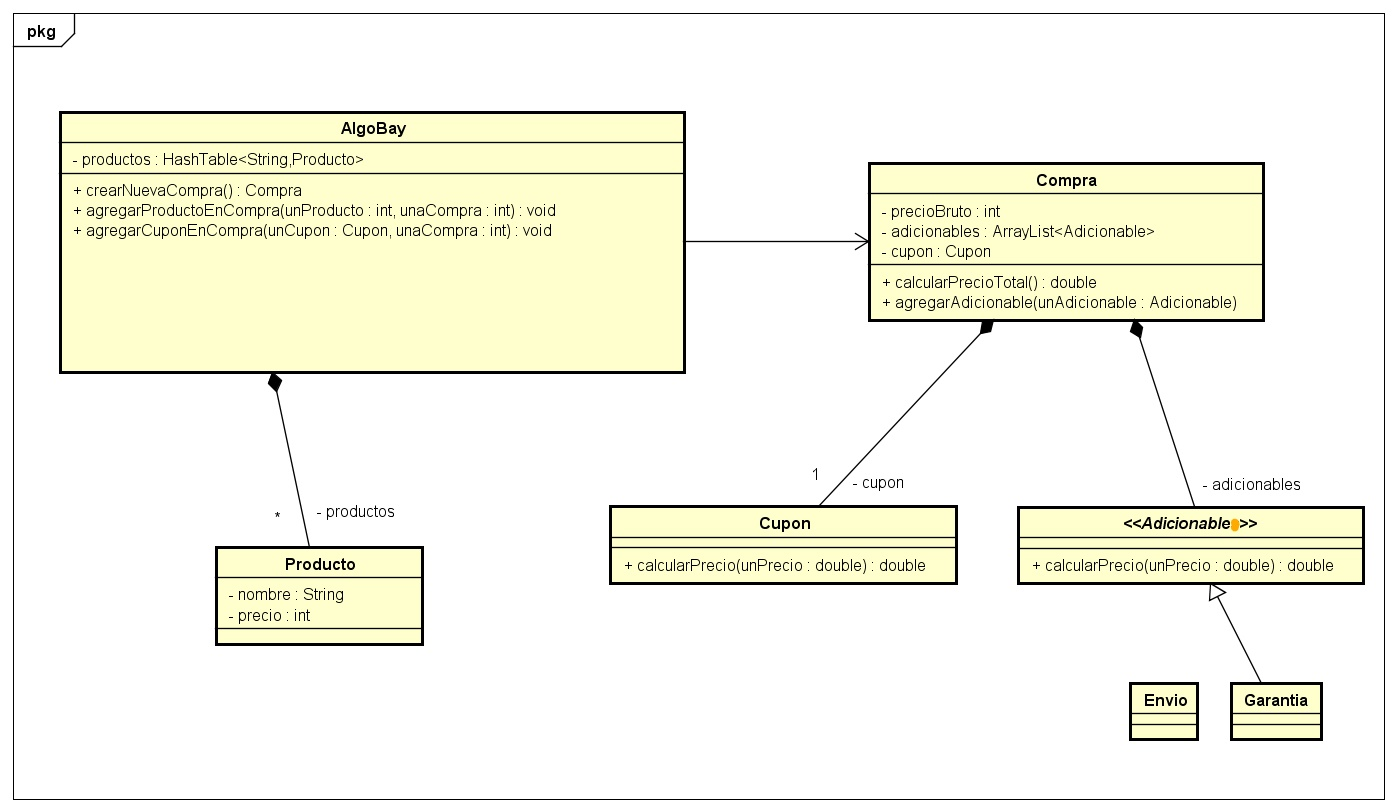
\includegraphics[width=1\textwidth]{0clases.jpg} 
\caption{\label{fig:class01}Diagrama conciso del programa.}
\end{figure}

\section{Detalles de implementación}\label{sec:implementacion}
% Explicaciones sobre la implementación interna de algunas clases que consideren que puedan llegar a resultar interesantes.

\subsection{AlgoBay}
AlgoBay, al actuar como moderadora, tiene una implementación bastante directa y sin desvíos, ya que en su mayoría se reduce a bajar el mensaje recibido. De recibir el deber de crear una compra, llama al constructor de compra. De recibir el deber de crear una compra con algun adicionable, llama no solo al constructor pero también a un metodo de esta que se encargue del labor. De esta forma se puede ver como, en sus métodos, delega la responsabilidad. Por ejemplo, al momento de crear un cupón y de agregarlo a una compra:

\begin{verbatim}
public Cupon crearCuponConPorcentaje(double unPorcentaje){
    return new Cupon(unPorcentaje);
}
\end{verbatim}

\begin{verbatim}
public void agregarCuponEnCompra(Cupon unCupon, Compra unaCompra){
    unaCompra.agregarCupon(unCupon);
}

\end{verbatim}

\subsection{Compra}
El mayor problema en la clase \textbf{Compra} fue la idea de dejar de lado el nombre del producto y que solo se encargue de sus precios, de esta forma haciendo que el precio de la compra, antes de aplicarle modificadores, sea una simple sumatoria. Una vez introducidos los modificadores, la decisión tomada fue la de armar una lista (\textbf{ArrayList}) de adicionables que, de ser el metodo \texttt{agregarAdicionable} invocado, irá llenando una lista de los adicionables de la compra, mientras que por otro lado se tenga una referencia al \textbf{único} cupón de esta. Teniendo esto, se puede calcular el precio total solamente invocando el método \textbf{calcularPrecio} sobre todos sus modificadores.

\begin{verbatim}
public double calcularPrecioTotal(){
	double precioTotal = precioBruto;
	for (Adicionable adicionable : adicionables)
			precioTotal = adicionable.calcularPrecio(precioTotal);
	if(cupon != null)
		precioTotal = cupon.calcularPrecio(precioTotal);
	return precioTotal;
}
\end{verbatim}

\subsection{Modificadores}
Lo complejo de los modificadores fue el hacer que cada uno pueda responder al mismo mensaje, el aplicado por compra, de manera distinta. Por lo tanto, se aplicó polimorfismo con herencia. De esta forma, \textbf{envío} y \textbf{garantía} implementan la interfaz adicionable mientras que el cupón actua independientemente y las tres contienen el mismo método, \textbf{calcularPrecio}, cada una aplicandolo de forma distinta. 

\begin{verbatim}
Envio >>> calcularPrecio
public double calcularPrecio(double unPrecio){
	if(unPrecio < 5000)
		return unPrecio+valor;
	return unPrecio;
}

Garantia >>> calcularPrecio
public double calcularPrecio(double unPrecio){
	return unPrecio*( (100+valor) /100);
}

Cupon >>> calcularPrecio
public double calcularPrecio(double unPrecio){
   return unPrecio - (unPrecio * (valor/100));
}
\end{verbatim}

Por otro lado fue complejo el comportamiento al momento de recibir más de un cupón para la misma compra, ya que estas solo deben tener uno, el mayor. Para esto, lo que se decidió fue que la clase de mercado simplemente llame al método de agregar un cupón a una compra y que la clase compra sea la que elija el mejor cupon para ella, que en este caso es el mayor. Para determinar si el cupon es el mayor, se llama al mensaje de cupón que lidia con eso: \textbf{esMayorQue}.

\begin{verbatim}
public boolean esMayorQue(Cupon otroCupon){
   return valor >= otroCupon.valor;
}
\end{verbatim}

\section{Excepciones}\label{sec:excepciones}
% Explicación de cada una de las excepciones creadas y con qué fin fueron creadas.

\begin{description}
\item[ProductoNoPresenteError] Teniendo el método \textbf{getProducto} para obtener un producto del mercado, si este no es encontrado, se lanzará esta excepción.
\item[ProductoPrecioNegativoError] Al agregar un producto al mercado, si este intenta ser agregado con un precio negativo, saltara esta excepción, ya que esto rompe el modelo planteado.
\item[CuponPorcentajeInvalidoError] Sea a la hora de crear un cupón de descuento, o de crear una garantía, si el valor no es un porcentaje valido, saltará esta excepción.
\end{description}

\section{Diagramas de secuencia}\label{sec:diagramasdesecuencia}
% Mostrar las secuencias interesantes que hayan implementado. Pueden agregar texto para explicar si algo no queda claro.

El primer diagrama de secuencia representa lo que pasa cuando se agregan productos al mercado y a su vez estos se agregan a una compra con envío, mostrando la interacción entre \textbf{AlgoBay} y \textbf{Compra} con \textbf{envío} (quien implementa de \textbf{<<Adicionable>>}). Luego, a esta compra se le pide el precio total.

\begin{figure}[H]
\centering
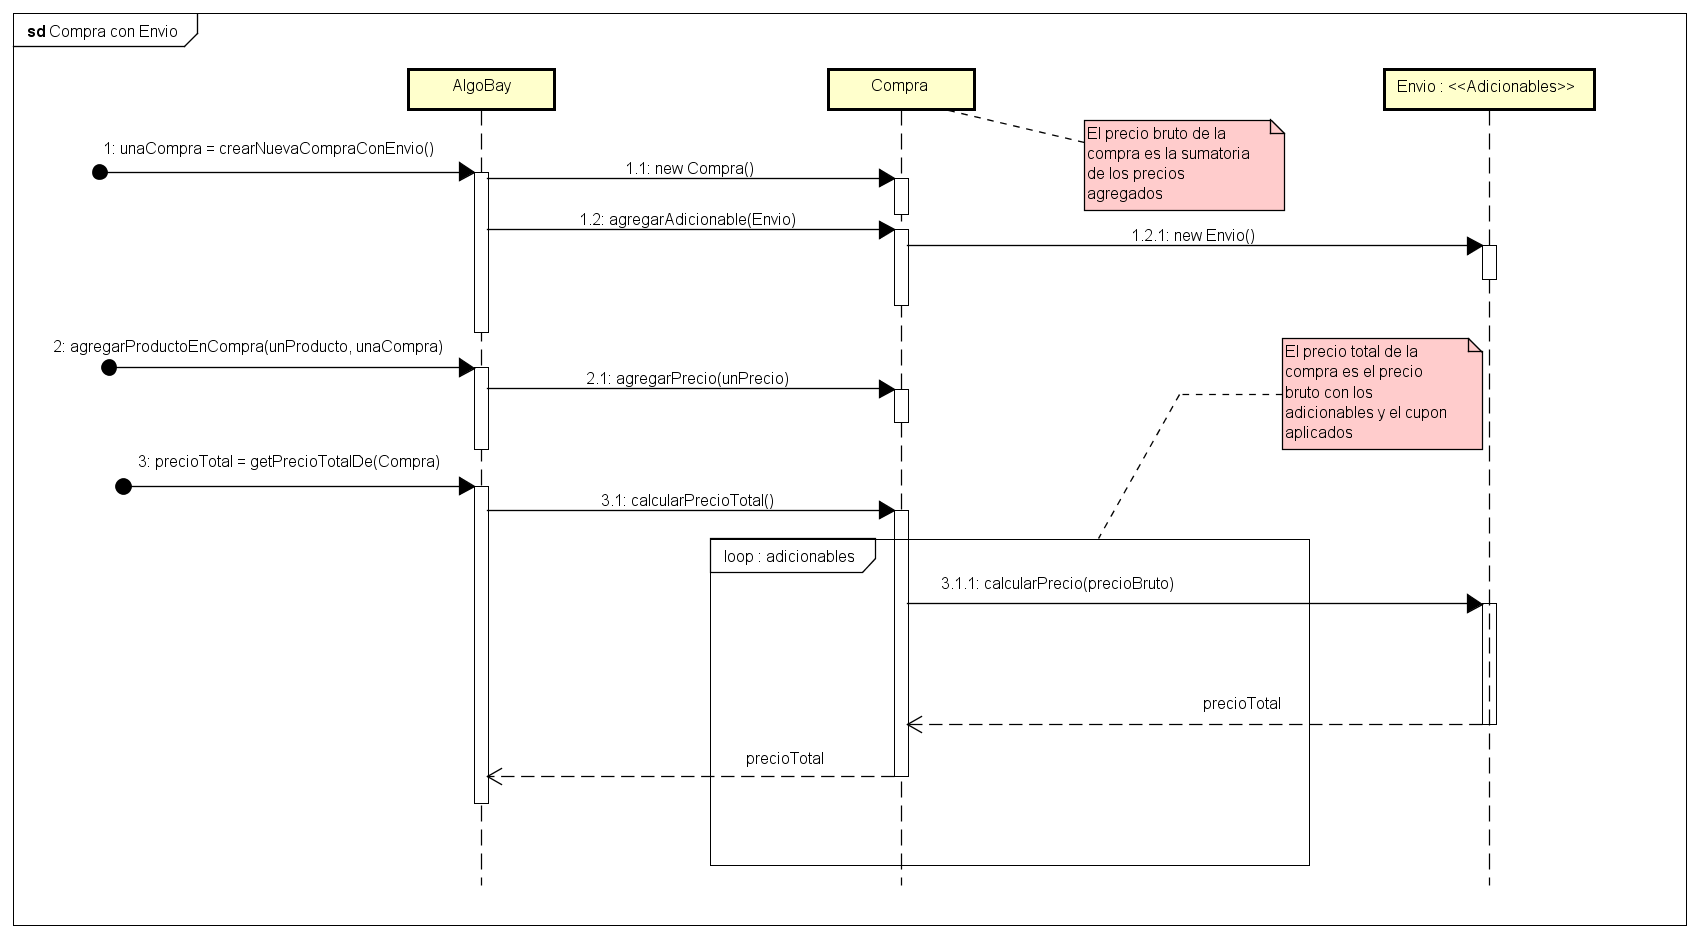
\includegraphics[width=0.9\textwidth]{1compraconenvio.png}
\caption{\label{fig:seq01}Comrpa con envío.}
\end{figure}

En el segundo diagrama de secuencia se ve como se comporta una compra a la que se le agreguen tanto un adicionable como un cupón
\begin{figure}[H]
\centering
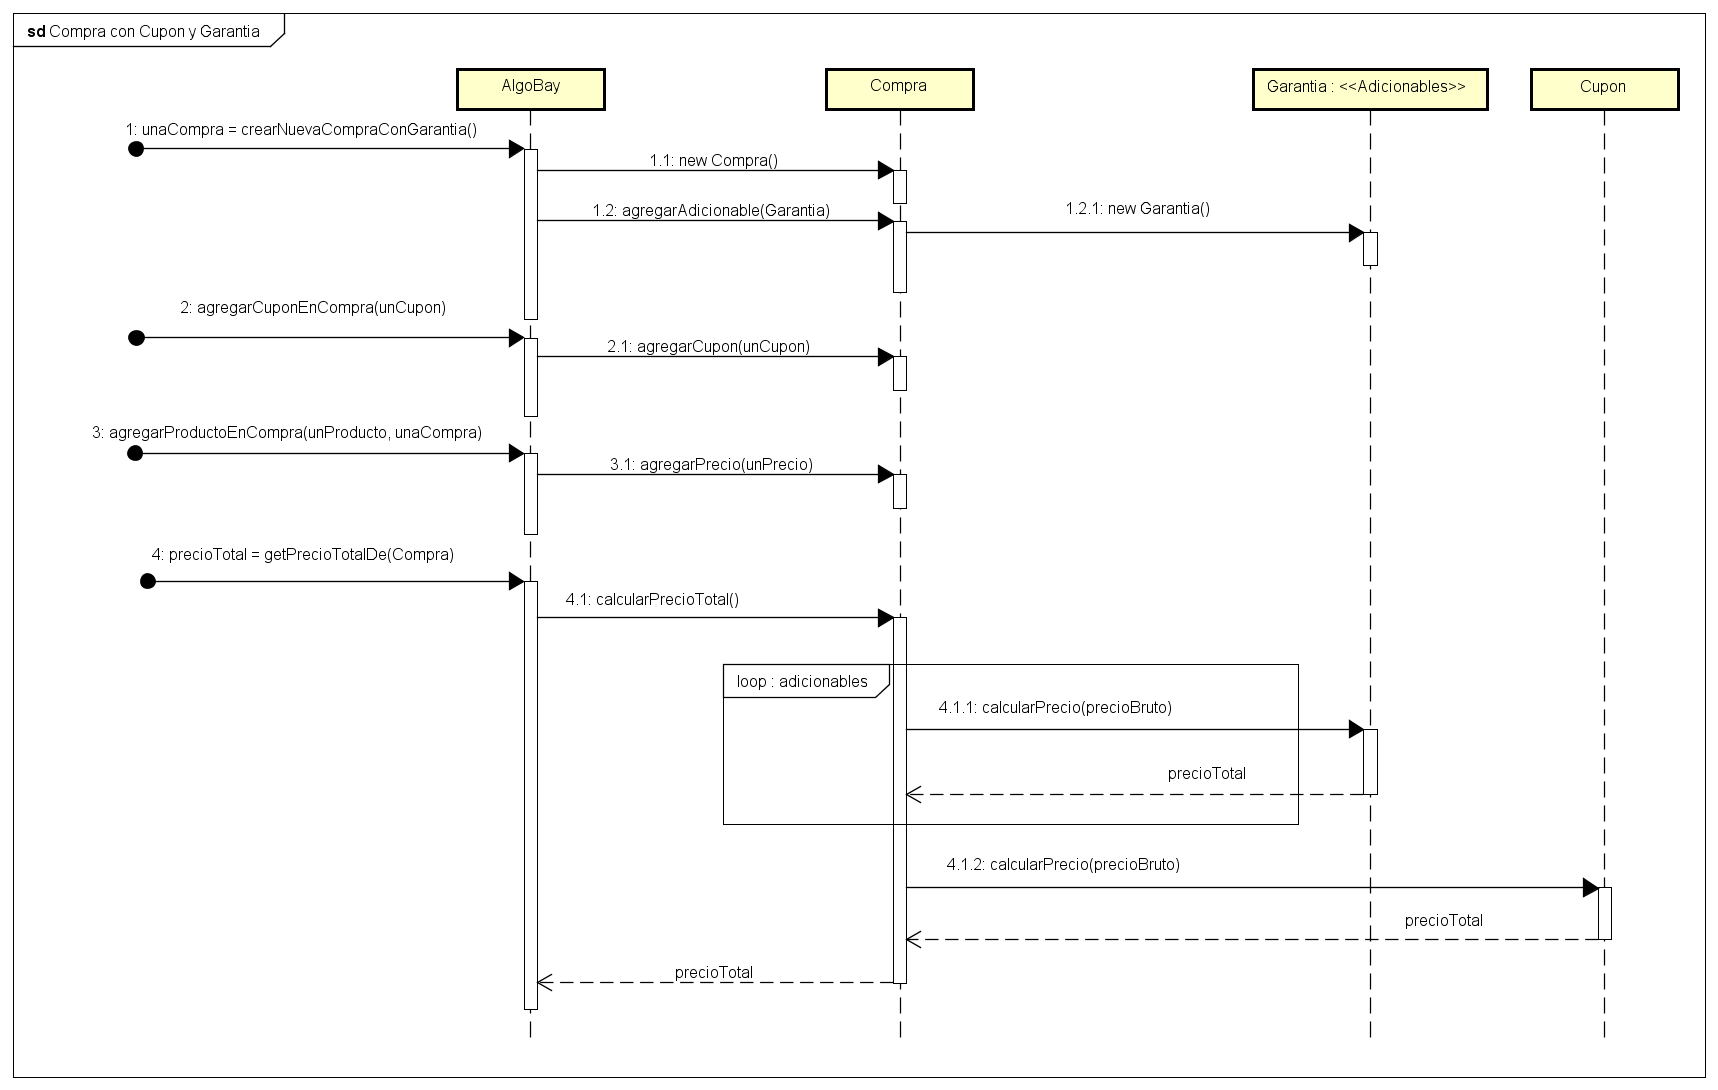
\includegraphics[width=1\textwidth]{2compraconenvioygarantia.png} 
\caption{\label{fig:seq02}Compra con garantía y cupón.}
\end{figure}

El último diagrama muestra como es la interacción entre \textbf{AlgoBay}, \textbf{Compra} y \textbf{Cupón} cuando se intenta de agregar más de un cupón a una compra, ya que el proceso de por sí es interesante por la delegación de responsabilidades

\begin{figure}[H]
\centering
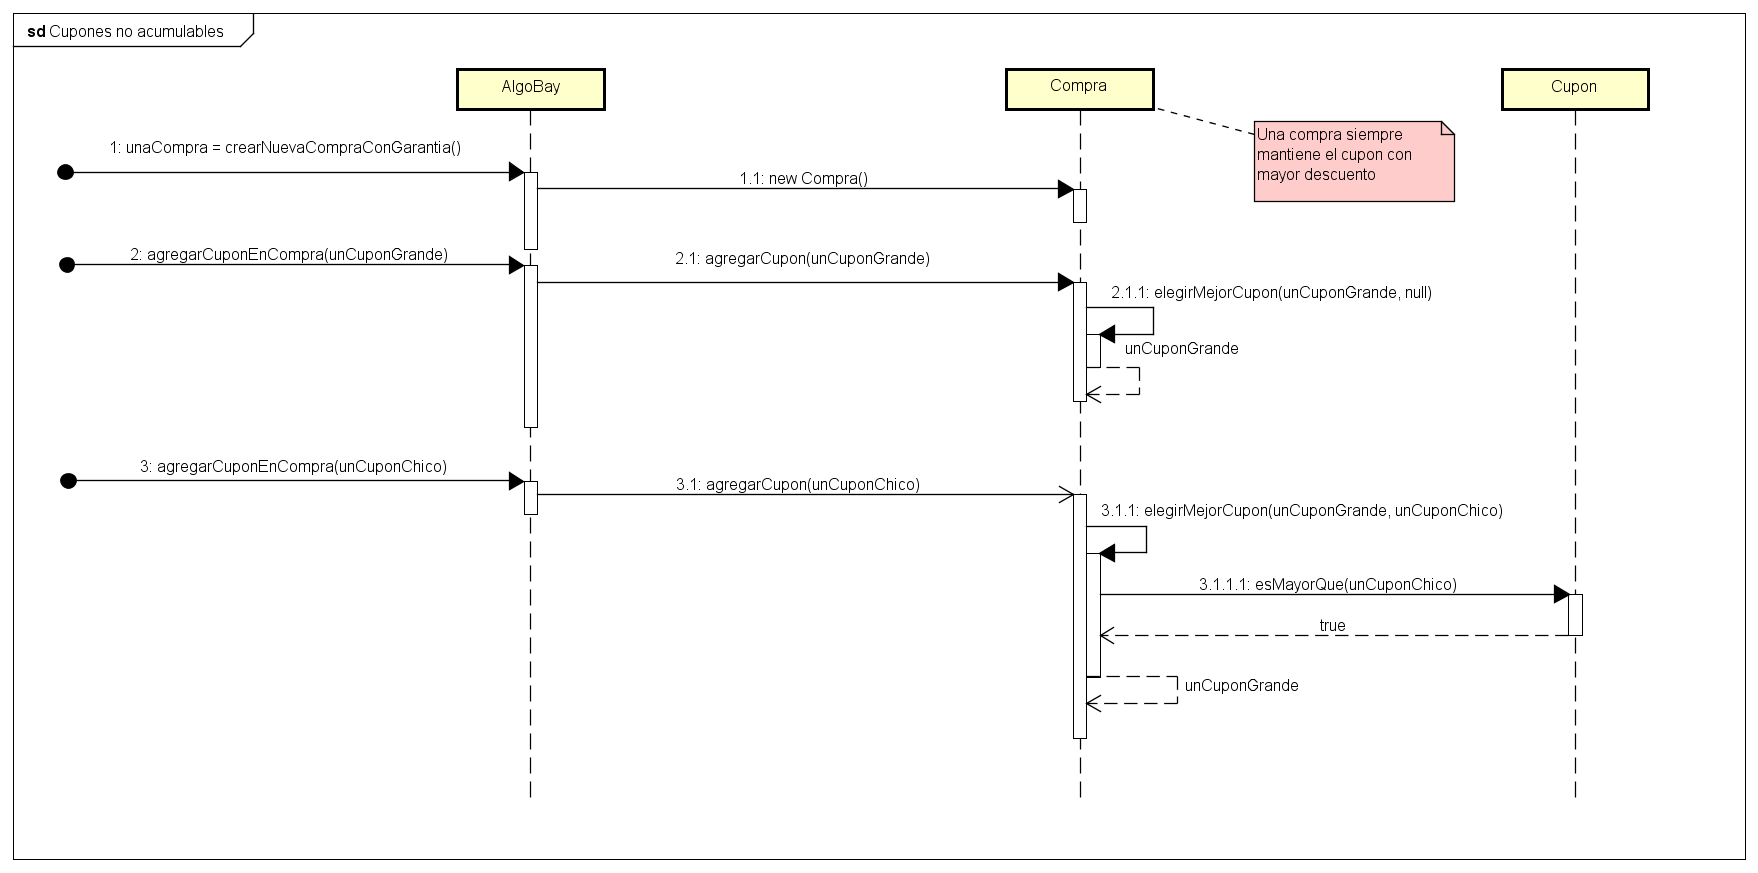
\includegraphics[width=1\textwidth]{3cuponesnoacumulables.png} 
\caption{\label{fig:seq03}Cupones no acumulables.}
\end{figure}


\end{document}
